\documentclass{beamer}
\usepackage{url}

\title{Quick Intro to Git version control}
%\author{Alexandre Beaulne}

\begin{document}

\begin{frame}
    \titlepage
\end{frame}

\begin{frame}
    \frametitle{Contents}
    \tableofcontents
\end{frame}

\section{Intro}

\begin{frame}
    \frametitle{Intro}
    \begin{center}
        Git is an open source, \textbf{distributed} version control
        system designed for speed and efficiency.
    \end{center}
\end{frame}

\begin{frame}
    \begin{figure}[h!]
        \frametitle{Centralized paradigm (CVS, SVN, Perforce)}
        \begin{center}
            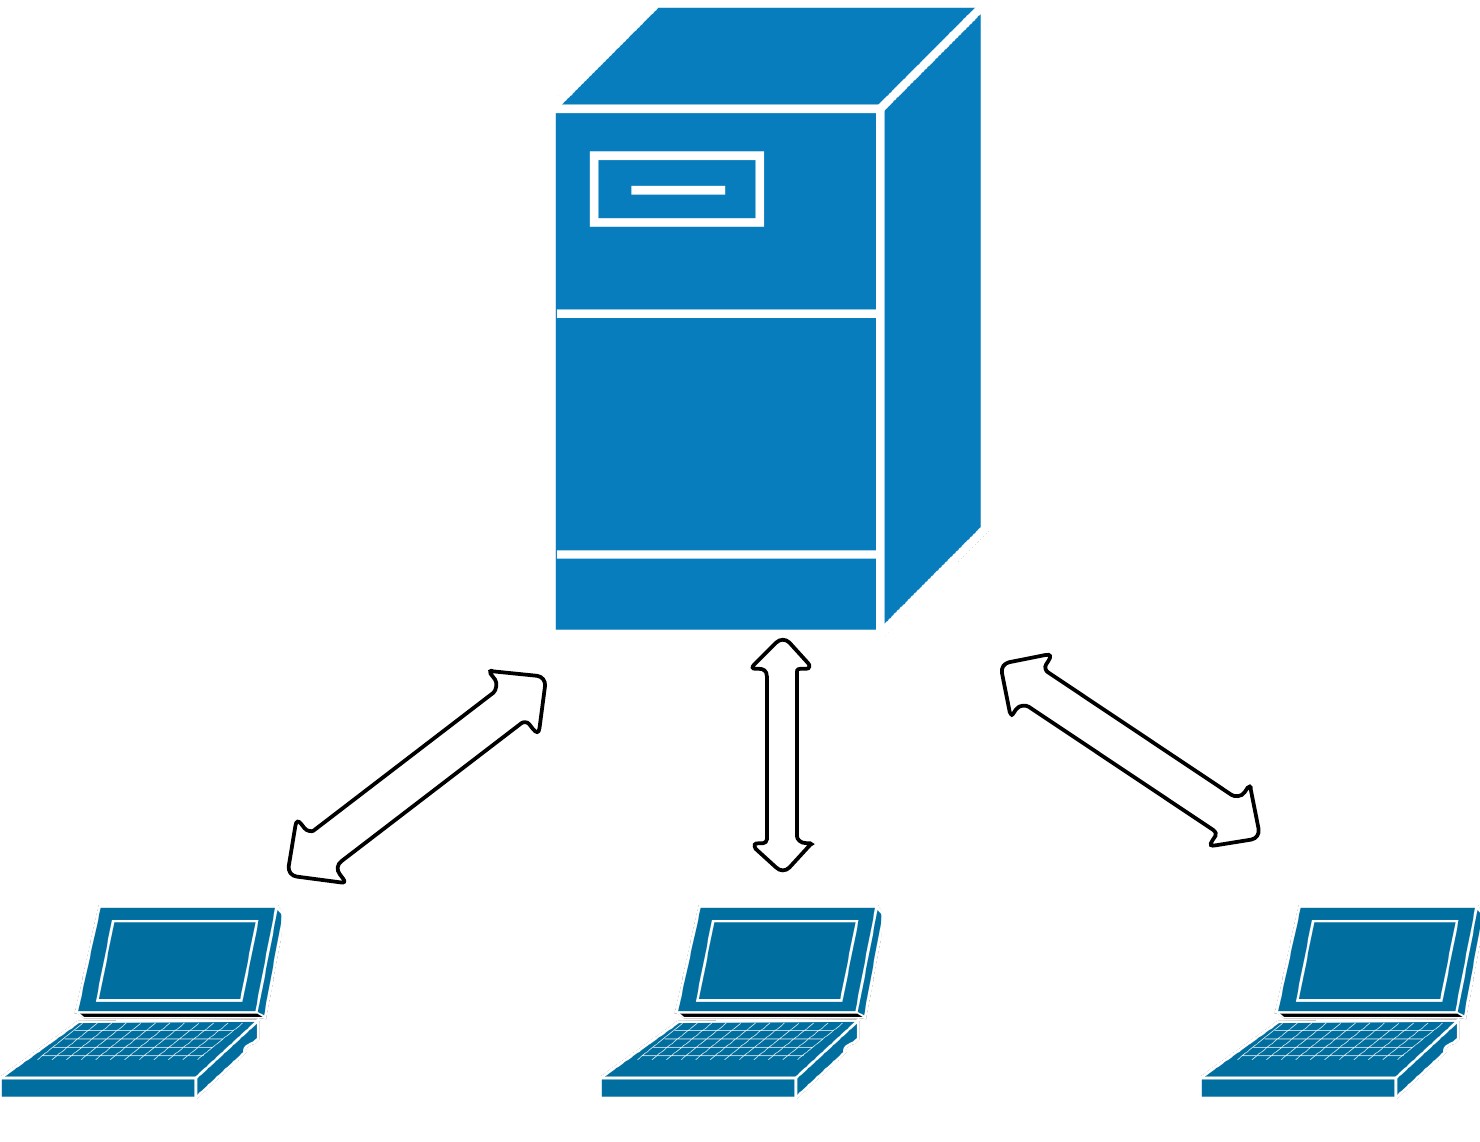
\includegraphics[scale=0.2]{centralized.png}
        \end{center}
    \end{figure}
\end{frame}

\begin{frame}
    \begin{figure}[h!]
        \frametitle{Distributed paradigm (Git, Mercurial)}
        \begin{center}
            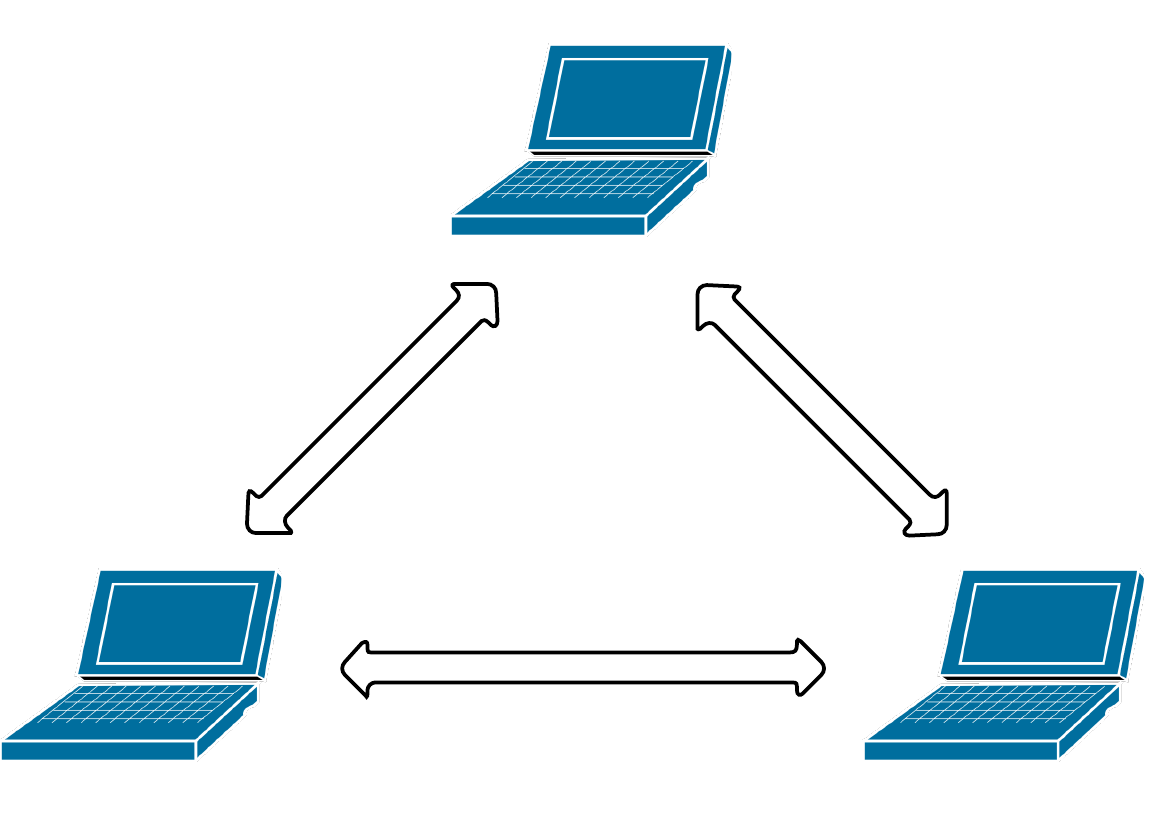
\includegraphics[scale=0.2]{distributed.png}
        \end{center}
    \end{figure}
\end{frame}

\section{Commands}

\begin{frame}
    \begin{figure}[h!]
        \begin{center}
            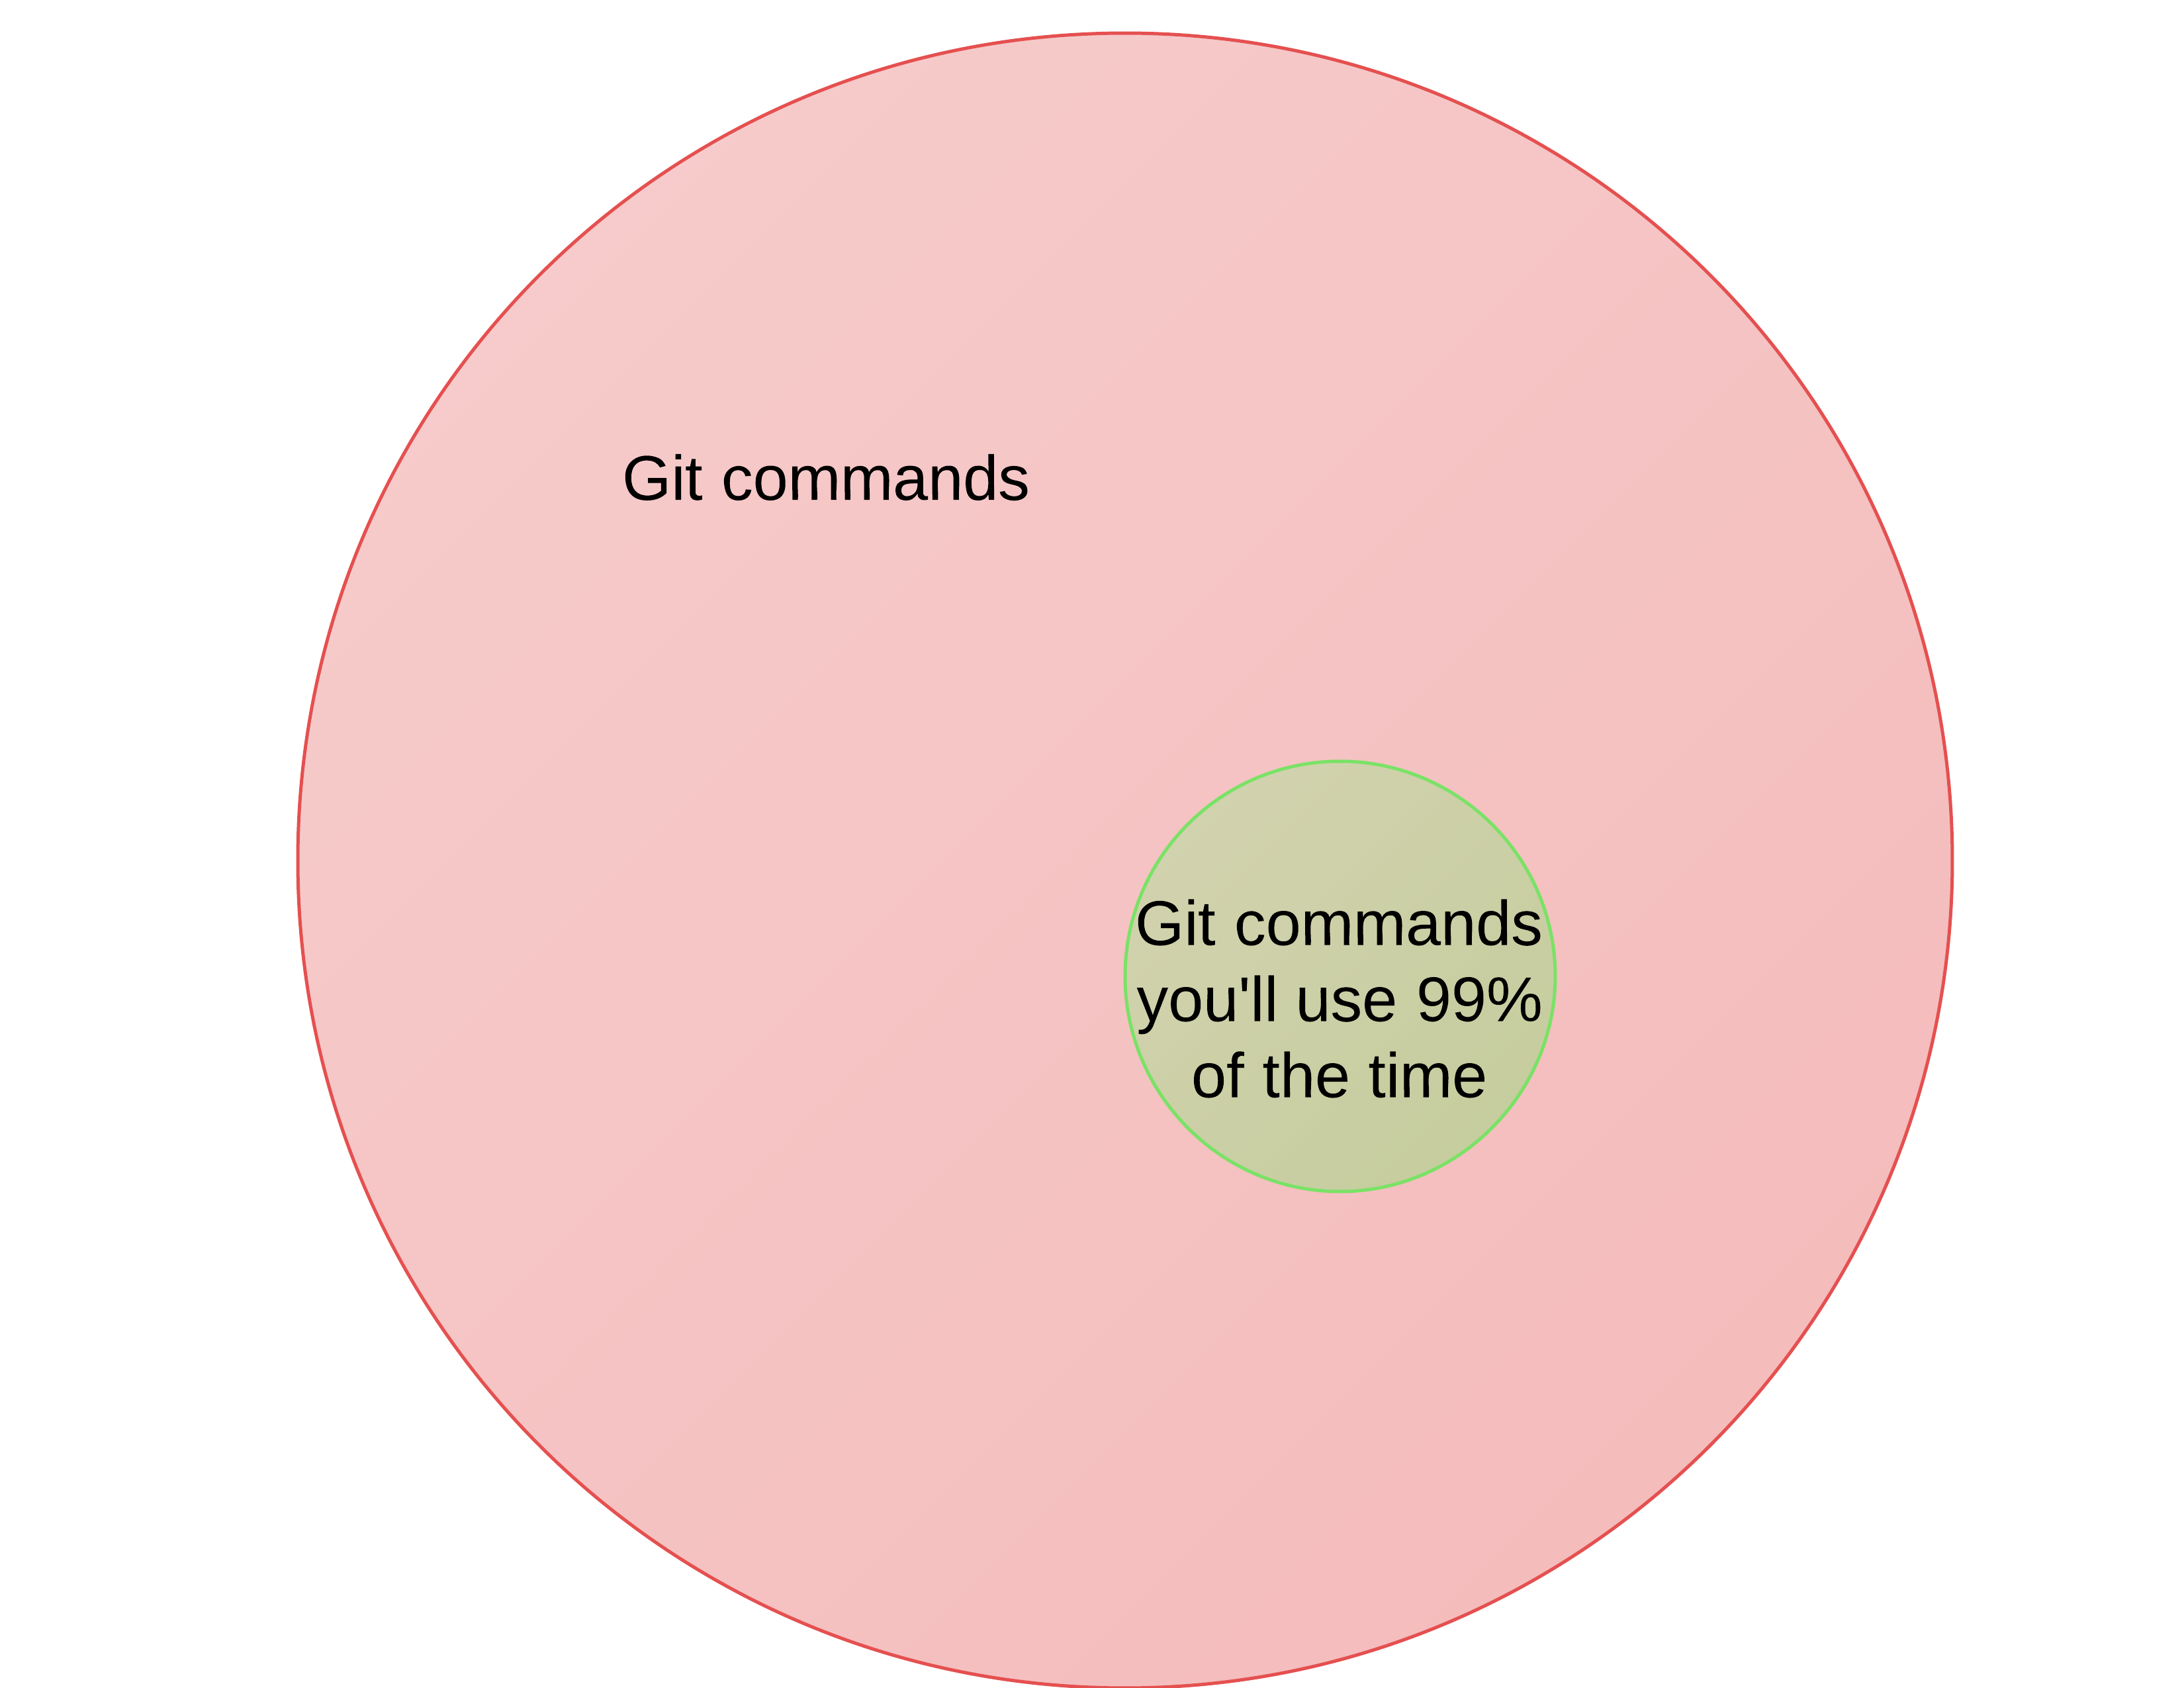
\includegraphics[scale=0.09]{git_commands1.png}
        \end{center}
    \end{figure}
\end{frame}

\begin{frame}
    \begin{figure}[h!]
        \begin{center}
            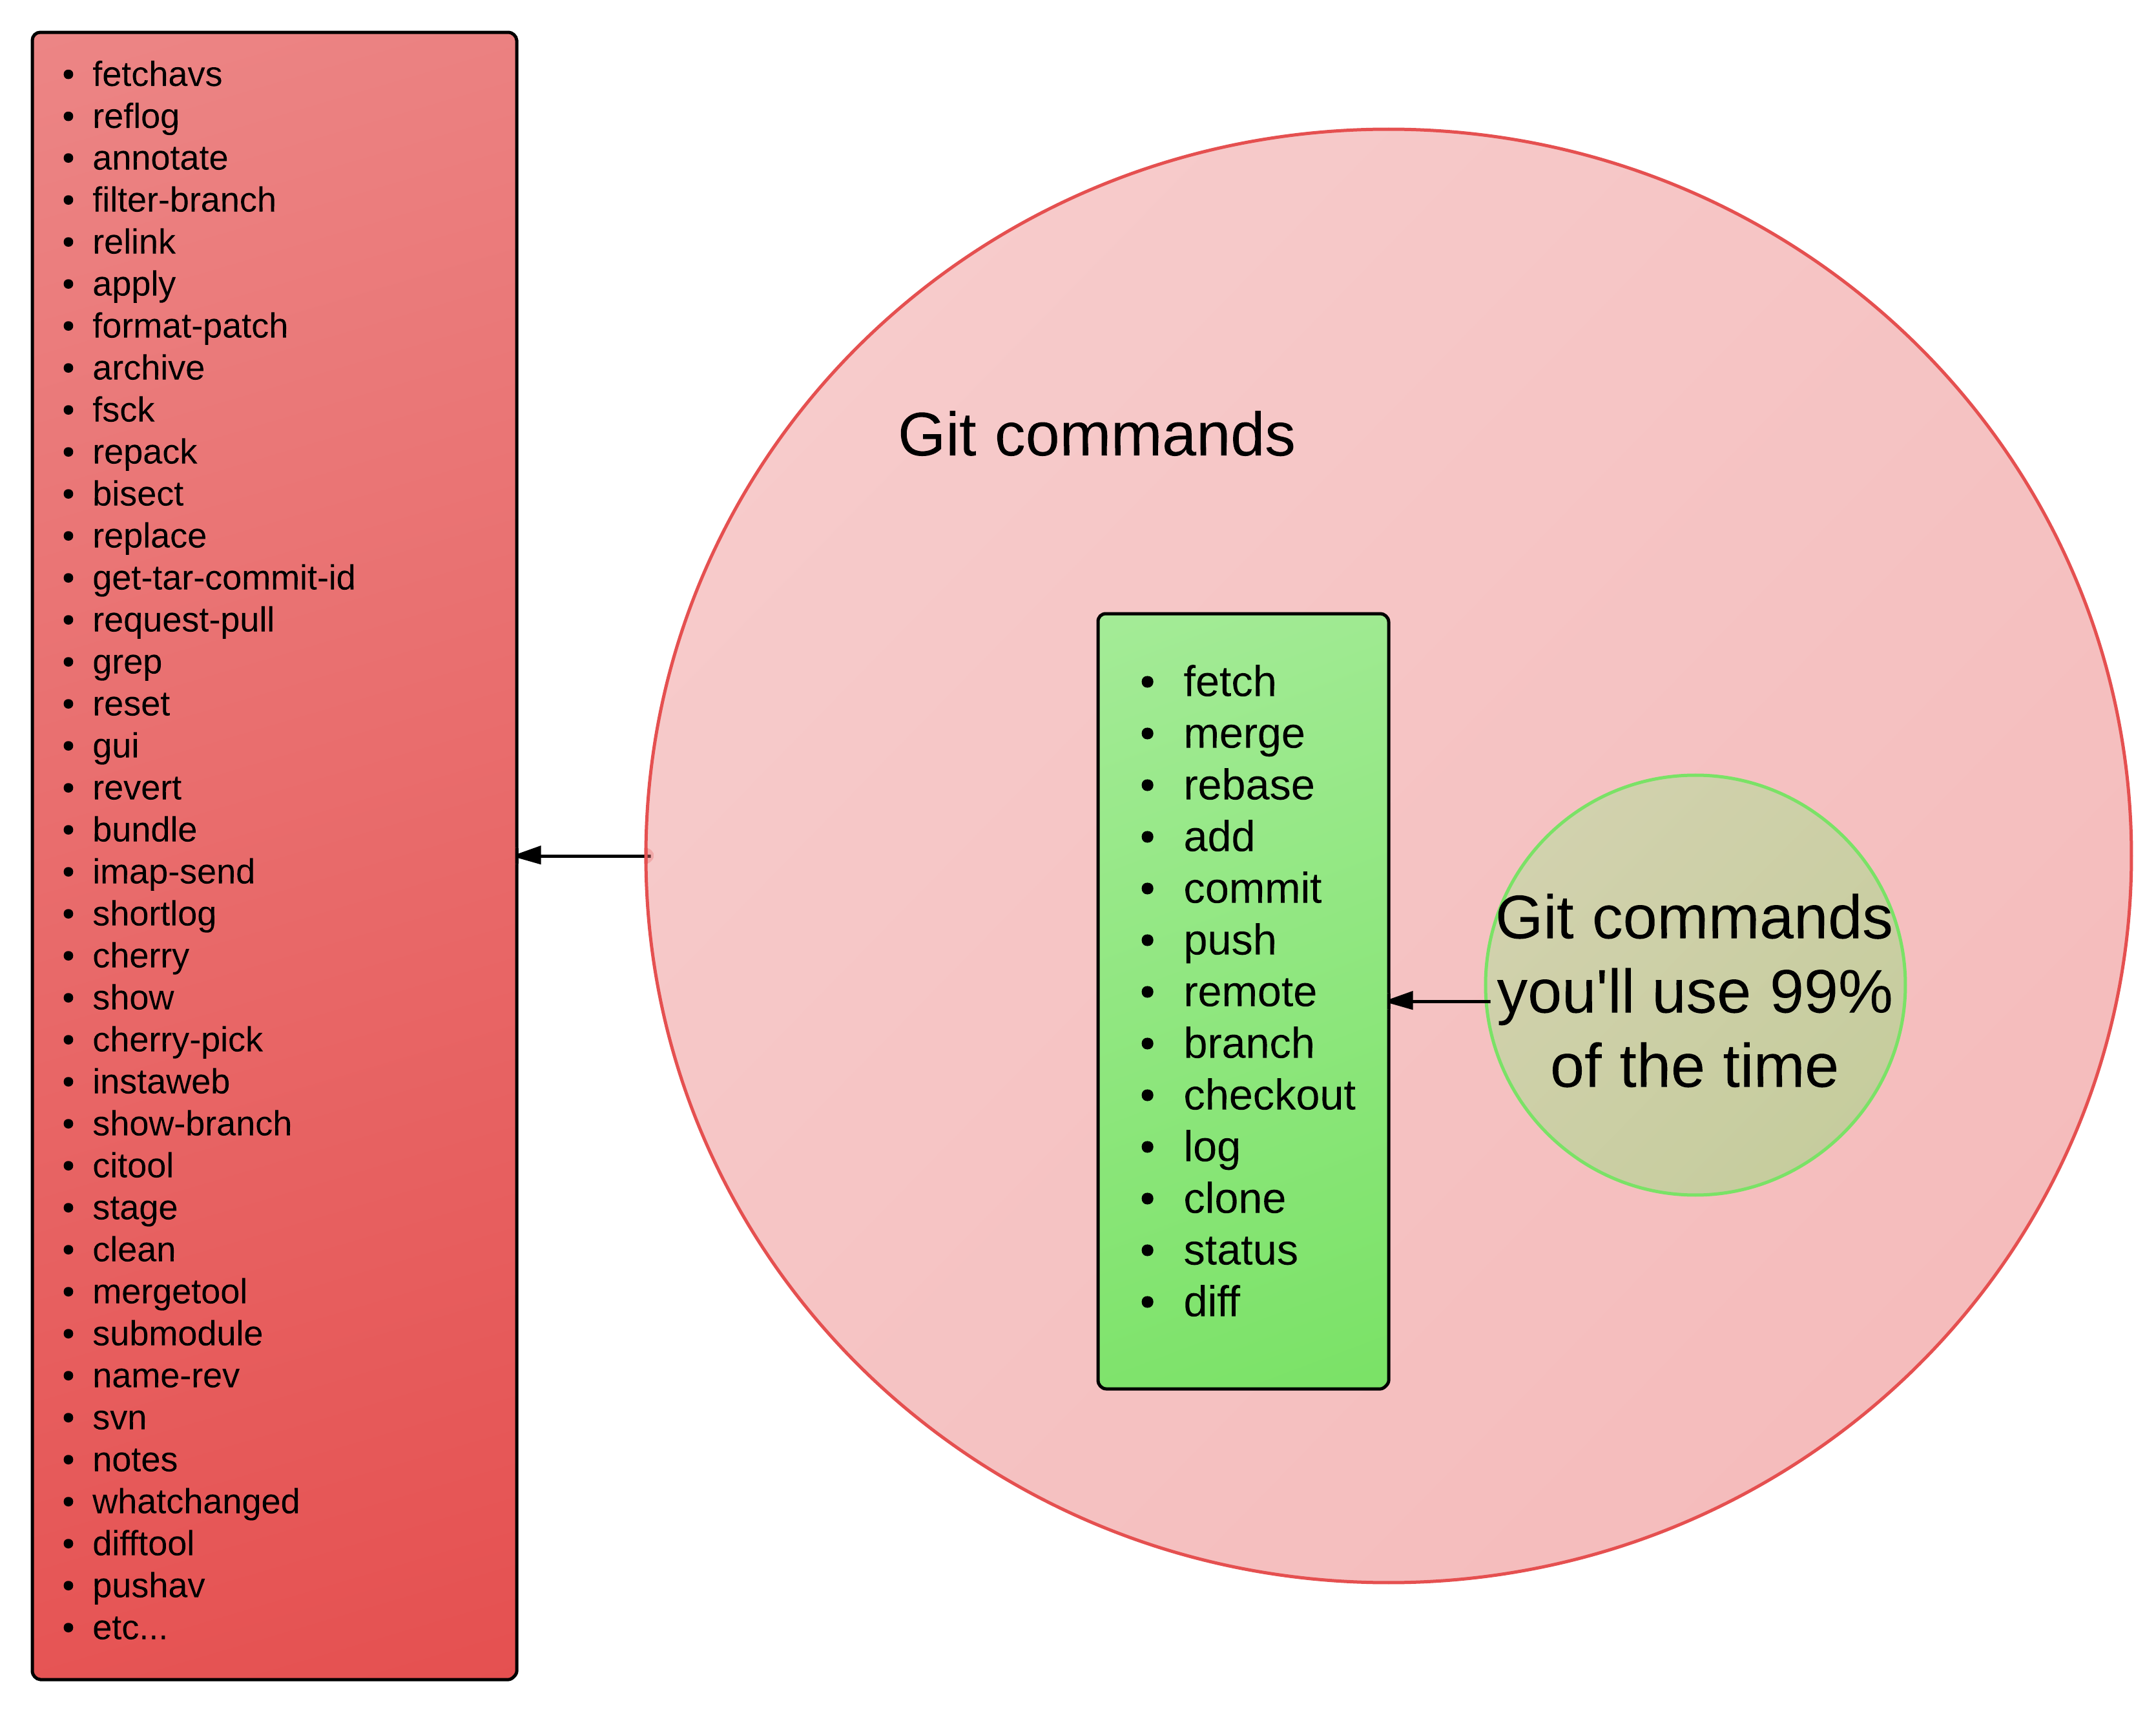
\includegraphics[scale=0.09]{git_commands2.png}
        \end{center}
    \end{figure}
\end{frame}

\section{Workflow}

\section{IDEs}

\section{Ressources}

\begin{frame}
    \frametitle{Ressources}
    \begin{center}
        Atlassian has a great straightforward tutorial at
        \url{https://www.atlassian.com/git/}
    \end{center}
\end{frame}

\section{Homework}

\end{document}

